%\documentclass[preprint]{aastex}  % USE THIS TO MAKE BIB, THEN FORMAT USING EMULATEAPJ
\documentclass[twocolumn,numberedappendix]{emulateapj}
\shorttitle{Fringe-Rate Filtering}
\shortauthors{Parsons, et al.}

\usepackage{amsmath}
\usepackage{graphicx}
\usepackage[figuresright]{rotating}
%\usepackage{rotating}
\usepackage{natbib}
%\usepackage{pdflscape}
%\usepackage{lscape}
\citestyle{aa}

\def\b{\mathbf{b}}
\def\k{\mathbf{k}}
\def\r{\mathbf{r}}
\def\q{\mathbf{q}}
\def\b{\mathbf{b}}
\def\kp{\mathbf{k}^\prime}
\def\kpp{\mathbf{k}^{\prime\prime}}
\def\V{\mathbb{V}}
\def\At{\tilde{A}}
\def\Vt{\tilde{V}}
\def\Tt{\tilde{T}}
\def\tb{\langle T_b\rangle}

\begin{document}
\title{Fringe-Rate Filtering}

\author{
Aaron R. Parsons\altaffilmark{1,2},
Adrian Liu\altaffilmark{1},
James E. Aguirre\altaffilmark{3},
Zaki S. Ali\altaffilmark{1},
David R. DeBoer\altaffilmark{2},
Daniel C. Jacobs\altaffilmark{8},
David F. Moore\altaffilmark{3},
Jonathan C. Pober\altaffilmark{1},
}

\altaffiltext{1}{Astronomy Dept., U. California, Berkeley, CA}
\altaffiltext{2}{Radio Astronomy Lab., U. California, Berkeley, CA}
\altaffiltext{3}{Dept. of Physics and Astronomy, U. Pennsylvania, Philadelphia, PA}
\altaffiltext{8}{School of Earth and Space Exploration, Arizona State U., Tempe, AZ}

\begin{abstract}
\end{abstract}

% XXX fringe weighting profile
% XXX delay spectrum not violated by freq-dependent fringe rate weights

\section{Introduction}

Further details are supplied in Appendices A and B of \citet{parsons_et_al2013}.

\begin{equation}
\tilde{V}(\tau)=\int{W(\nu)\cdot S(\nu)\cdot V(\nu)e^{-2\pi i\nu\tau}~d\nu},
\label{eq:dtransform}
\end{equation}

\section{Fringe-Rate Filtering}
\label{sec:fringe_rate_filtering}
%fringe_rate_filter.py -C psa898_v002 -a cross --clean=1e-2 --minfr=-1 --fr_frac=1.2 

In the last step prior to forming power spectra,
we apply a fringe-rate filter to effect time-domain integration,
using the effective time interval that a baseline measures a single $k$-mode to integrate coherently
(with noise decreasing
as $\sqrt{t}$, in units of mK), before measurements at different times represent independent modes
that must be squared before further integration (with noise now decreasing as $\sqrt{t}$, in units of mK$^2$).

One way of handling this additional integration is via gridding in the $uv$-plane.
Each measured visibility in a wide-field interferometer represents the integral over a kernel in
the $uv$-plane that reflects the primary beam of the elements \citep{bhatnagar_et_al2008,morales_matejek2009} and the $w$ component 
of the baseline \citep{cornwell_et_al2003}.  As noted in
\citet{sullivan_et_al2012} and \citet{morales_matejek2009},
in order to optimally account for the mode-mixing introduced by these kernels, gridding kernels must be
used that correctly distribute each measurement among the sampled $uv$-modes, such that, in the ensemble average
over many measurements by many baselines, each $uv$-mode becomes an optimally weighted estimator of the actual
value given the set of measurements.

However, this approach has a major shortcoming when applied to maximum-redundancy array configurations.
In order
to maximize sensitivity, such
configurations are set up to deliberately sample identical visibilities that reflect the same 
combinations of modes in the $uv$ plane, with few nearby measurements (P12a).  As a result,
such array configurations tend to lack enough measurements of different combinations of $uv$ modes
to permit the ensemble average to converge on the true value.  Said differently, maximum-redundancy
array configurations tend to produce measurement sets that, when expressed as linear combinations
of $uv$-modes of interest, are singular.

Our alternative approach avoids this and many of the difficulties outlined
in \citet{hazelton_et_al2013} by applying a carefully tailored
fringe-rate filter to each time series of visibility spectra.  As outlined in Appendix \ref{app:data_compression}
in the context of data compression, we
take the Fourier transform of the time series in each channel and apply a low-pass filter that preserves
fringe-rates that geometrically correspond to sources rotating on the celestial sphere.  
For a planar array with transit observations, fringe-rates vary according to declination, with fringe rates
reaching a maximum ($f_{\rm max}$) at 
$\delta=0^\circ$, decreasing to 0 at $\delta=-90^\circ$, and for an array such as PAPER deployed near
-30$^\circ$ S latitude, reaching a minimum of $\approx-f_{\rm max}/2$ at $\delta=-60^\circ$ on
the far side of the south celestial pole.
In order to
avoid introducing undesirable frequency structure, we apply the same filter, tuned to the width
set by the highest frequency of the sub-band used in the
power spectrum analysis described
in \S\ref{sec:dspec_crossmult}, to each channel,
even though maximum fringe-rates are generally frequency-dependent.
%Since fringe rates are a
%natural basis for celestial emission
%over short time intervals, fringe-rate
%filters can be narrowly tailored to the geometric bounds of a baseline.
%In contrast, simply summing integrations over an equivalent time interval 
%(corresponding to a sinc filter in fringe-rate space) will tend to significantly suppress emission at
%fringe rates that geometrically correspond to the sky.
In a future paper, we will explore the idea
of employing fringe-rate filters that purposely down-weight fringe-rate modes on the sky according to
the expected signal-to-noise ratio in each mode.  Such filters would essentially correspond to a
one-dimensional implementation of the inverse primary beam $uv$-gridding discussed in \citet{morales_matejek2009},
and have many features in common with m-mode synthesis described in \citet{shaw_et_al2013}.

Since thermal noise scatters equally into all fringe rate bins, applying a filter
that passes only fringe rates corresponding the celestial emission has the effect of de-noising the data.
We apply such a filter to the data, choosing the bounds of the filter to match the geometric
bounds set by a 30-m east-west baseline, according to the equation
\begin{equation}
f_{\rm max} = \frac{|\b_{\rm eq}|}{c} \omega_\oplus \nu,
\label{eq:fringe_rate}
\end{equation}
where $f_{\rm max}$ is the maximum fringe rate, 
$\b_{\rm eq}$ is the baseline vector projected parallel to the equatorial 
plane, $c$ is the speed of light,
$\omega_\oplus$ is the angular frequency of the Earth's rotation,
and $\nu$ is the spectral frequency. 
% 780 = 30e2 / c * 2pi / 86164 * .174, where .174 is chosen because want to not attenuate sky over entire band
At 174 MHz (the highest frequency in a 20-MHz window centered on 164 MHz that is used in \S\ref{sec:dspec_crossmult}),
$f_{\rm max}=1.3$ mHz, corresponding to a fringe period of 780 s.  Hence, the fringe-rate filter that is
applied passes fringe-rates in the range $-0.7<f<1.3$ mHz.  The width of this filter corresponds in 
sensitivity to an effective integration time of 525 s.
We note that
this filtering could have been applied during the data compression described in \S\ref{sec:preprocessing},
but was implemented separately to enable the compression to work uniformly
over all baselines in the array without additional information about antenna location.

After applying this filter,
we transform the data back to time domain in preparation for forming power spectra via the delay transform.
It should be noted that, in time domain, the data are now heavily over-sampled; adjacent samples are no longer
statistically independent.  Hence, when averaging power-spectra versus time,
noise will not beat down according to the strict number in samples, but rather, according to
the actual number of statistically independent samples underlying the time series.

\begin{equation}
\widehat P(\k_{t\tau}) = \left(\frac{\lambda^2}{2k_{\rm B}}\right)^2\frac{X^2Y}{\Omega B}
\left\langle{\tilde V_i(\tau,t) \tilde V_j^*(\tau,t)}\right\rangle_{i<j},
\label{eq:pspec_cosmo}
\end{equation}
which follows from equation 12 of P12a, with $\lambda$ being the observing
wavelength, $k_{\rm B}$ is Boltzmann's constant, $X^2Y$ is a cosmological scalar with units
of $\frac{h^{-3}\ {\rm Mpc}^3}{{\rm sr}\cdot {\rm Hz}}$, $\Omega$ is the angular 
area\footnote{
As described in detail in Appendix \ref{app:beam_area}, the angular area used to normalize
high-redshift 21cm power spectrum measurements (e.g., $\Omega$ in Equation \ref{eq:pspec_cosmo}) is proportional
to the integral of the squared beam power over angular area ($\Omega_{\rm PP}$; equation \ref{eq:beam_squared}).
This contrasts the standard beam area ($\Omega_{\rm P}$; equation \ref{eq:beam_area}) that is
used to relate flux density to a brightness temperature.
Since Equation \ref{eq:pspec_cosmo} 
relates a measured visibility in units of brightness
temperature to $P(\k)$, a factor of $\Omega_{\rm P}^2$ has already been
applied to convert Jy to mK.  In this case,
$\Omega$ indicates the remaining factor of $\Omega_{\rm PP}$, which for PAPER is 0.31 sr.},
$B$ is the bandwidth, $\langle\dots\rangle_{i<j}$ indicates the ensemble average
over instantaneously redundant baseline measurements indexed by $i,j$,
and $\tilde V(\tau,t)$ is the delay-transformed visibility,
expressed in terms of delay $\tau$ and time $t$.
We use $t$ as a subscript on $\k$
to denote the different modes sampled by a baseline as the sky rotates, and $\tau$ to indicate
the dependence of $\k$ on the delay mode in question.

\begin{equation}
\widehat \Delta^2_{21}(k) = \frac{k^3}{2\pi^2}\left\langle \widehat P(\k_{t\tau})\right\rangle_{|\k_{t\tau}|=k},
\end{equation}
where the three-dimensional symmetry of the power spectrum is invoked to average over
all independent measurements of modes in a shell of $|\k|=k$, with independent measurements
indexed here by $t$.  As described in \S\ref{sec:fringe_rate_filtering}, the number of independent modes
that are averaged (with noise decreasing with number of modes, $M$, as $\sqrt{M}$ in mK$^2$ units; see P12a) is 
determined
by overall observing window and the number of fringe-rate bins that are 
preserved in the fringe-rate filtering process.
Since we have not decimated the number of integrations to the critical sampling rate corresponding to the 
width of the applied fringe-rate filter, $M$ is {\it not} the number of integrations.  However,
we are free to average the power spectrum estimates for each integration, even though nearby samples
do not have statistically independent noise, understanding that noise will decrease according to the number
of underlying independent samples.

\subsection{Crosstalk}

Crosstalk removal proceeds by subtracting the
1-hr time-average of the visibilities for each baseline from each integration.  This process,
described in \citet{parsons_et_al2010}, distinguishes oscillating fringes associated with 
celestial emission from the static phase bias associated with crosstalk. This crosstalk-removal
filter essentially constitutes a high-pass fringe-rate filter, as described in \S\ref{sec:fringe_rate_filtering}.
The width of the stop-band of the crosstalk filter is much narrower than low-pass fringe-rate filters described in
that section.
Nighttime data are averaged in LST over the 55-day observation using 43-second
time bins matching the integration interval of the data after the compression step described
in \S\ref{sec:preprocessing}.


\section{Simulations}
\label{sec:sim}

\subsection{Point Source Simulations for Mapping Beam Response}
\label{sec:sim_pnt}

\subsection{Noise Simulations for Estimating Signal Loss}
\label{sec:sim_nos}

Describe the simulations here.

\section{Beam Sculpting}
\label{sec:bmsculpt}

\begin{figure*}\centering
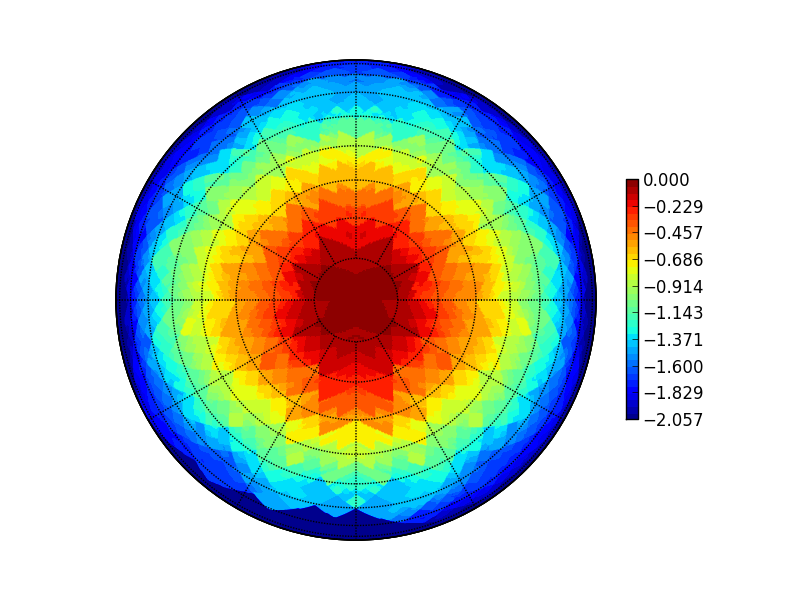
\includegraphics[width=.6\columnwidth]{plots/beam_raw.png}
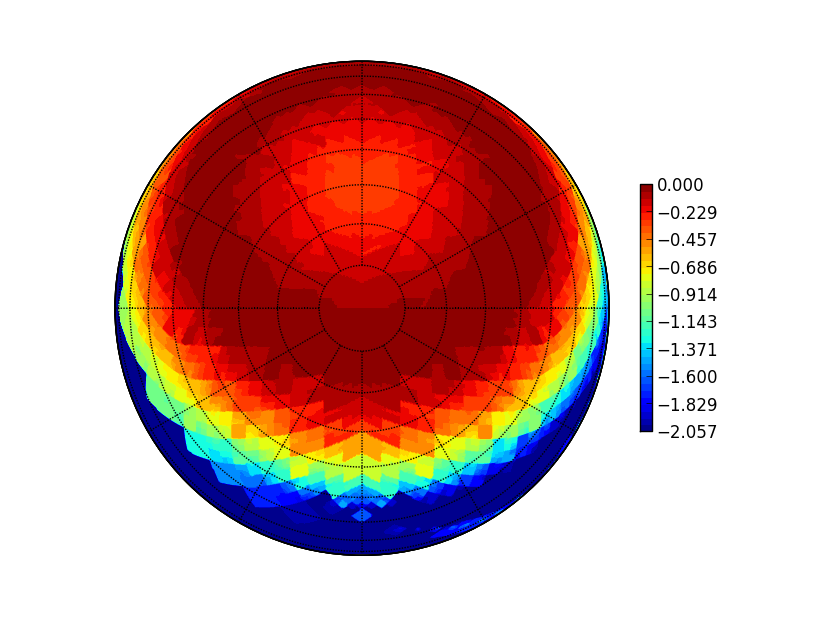
\includegraphics[width=.6\columnwidth]{plots/beam_wgt.png}
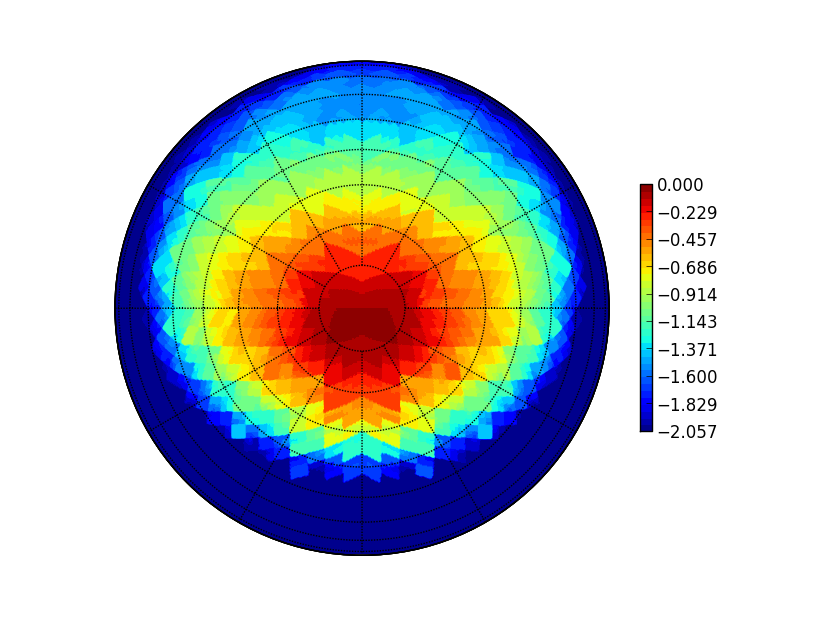
\includegraphics[width=.6\columnwidth]{plots/beam_fng.png}
\caption{
The effective primary beam response of a baseline, as determined from the simulations in \S\ref{sec:sim_pnt}.
Panels indicate reconstructions of PAPER's model beam response used in the simulation (left), the 
beam weighting that results from the application of a fringe-rate filter weighted to optimize SNR for
a 30-m baseline with PAPER's beam response (center), and the effective primary beam response of the
baseline after the application of the fringe-rate filter.
}\label{fig:}
\end{figure*}


\section{Matching Polarization Beams}
\label{sec:polbeams}

\section{Results and Discussion}
\label{sec:results}

\section{Conclusion}
\label{sec:conclusion}

\section{Acknowledgment}

% ---------------------------------------------------------------------
% ---------------------------------------------------------------------
% ---------------------------------------------------------------------

Similar geometric limits apply to the variation of visibilities in the time dimension.  As
described in Equation 7 of \citet{parsons_backer2009}, the rate of change of the geometric delay versus
time --- that is, delay-rate --- is given by
\begin{equation}
\frac{d\tau_g}{dt}=-\omega_\oplus\left(\frac{b_x}{c}\sin H + \frac{b_y}{c}\cos H\right)\cos\delta,
\end{equation}
where $\b=(b_x,b_y,b_z)$ is the baseline vector expressed in equatorial
coordinates, $\omega_\oplus$ is the angular frequency of the earth's rotation, and $H,\delta$ are the
hour-angle and declination of a point on the celestial sphere, respectively.  As a result, there exists a maximum
rate of change based on the length of a baseline projected to the $z=0$ equatorial plane.
For arrays not deployed near the poles, $|b_y|\gg|b_x|$ (i.e.,
they are oriented more along the east-west direction than radially from the polar axis),
and the maximum rate of change corresponds to $H=0$ and $\delta=0$, where we have
\begin{equation}
-\omega_\oplus\frac{|b_y|}{c}\le\frac{d\tau_g}{dt}\le\omega_\oplus\frac{|b_y|}{c}.
\end{equation}
For a maximum east-west baseline length in the PAPER array of 300m, $\omega_\oplus|b_y|/c$ is approximately
0.07 ns/s.  
To better elucidate the meaning of this bound, we take the Fourier transform 
along the time axis (see Equation 8 in \citealt{parsons_backer2009}) for a model visibility
consisting of a single point source located at the point of maximum delay-rate, which gives us
\begin{align}
\Vt(\nu,f)&\approx\At(\nu,f) * \tilde{S}(\nu) * \int{e^{2\pi i\omega_\oplus\frac{b_y\nu}{c}t}e^{-2\pi ift}dt}\nonumber\\
&\approx\At(\nu,f) * \tilde{S}(\nu) * \delta_{\rm D}(\frac{b_y}{c}\omega_\oplus \nu - f),
\end{align}
where $f$ is the fringe-rate of the 
source\footnote{Delay rate is equivalent to the frequency-integrated fringe rate.}, 
$\At(\nu,f)$ indicates the Fourier transform of the antenna response along the time direction,
and approximation is
indicated because we assume $|b_y|\gg|b_x|$, and because the Fourier transform must involve
a discrete length of time, during which our assumption that $\cos H\approx1$ breaks down at second order.
The delta function above gives rise to the expression for the maximum fringe rate in Equation \ref{eq:fringe_rate}.

This example of a source with a maximal fringe-rate serves to show that a 
filter may be applied in delay-rate domain, using the fact that the maximum
delay-rate is bounded by the maximum fringe rate within the band (i.e. evaluating Equation \ref{eq:fringe_rate}
at the maximum $\nu$ involved in the delay transform), to remove emission that exceeds the variation
dictated by array geometry for sources locked to the celestial sphere.  As in the delay filtering case, assuming
the geometric bounds on delay rate implicitly assumes that $\At$ and $\tilde{S}$ are compact in $f$, which
is to say that instrumental responses and celestial emission must be smooth in time; variable
emission from, e.g., fast-transients will be heavily suppressed by such delay-rate filters.
For PAPER, with a maximum baseline length of 300m and a maximum observing frequency of 200 MHz, 
the maximum delay-rate has a period of 68.5s.  As described in \S\ref{sec:fringe_rate_filtering}, at PAPER's
latitude, delay-rates range from -$f_{\rm max}/2$ to $f_{\rm max}$.  Filtering delay-rates to this
range corresponds in sensitivity to an effective integration time of 45.2 s.
An example of the bounds of a delay filter in DDR space is given
by the shaded magenta region in Figure \ref{fig:ddr_compression}.  As in the delay filtering case,
filtering along the delay-rate axis permits substantial down-sampling of the signal, which is
the basis for the reduction in data volume along the time axis.
We note that for the analysis
in \S\ref{sec:preprocessing}, we choose to use a slightly wider delay-rate filter to be conservative in
our first application of this technique, corresponding to an integration time of 43 seconds.

\section{On Calculating Beam Areas for Normalizing Power-Spectrum Measurements}
\label{app:beam_area}

We begin by examining the integrated volume, $\mathbb{V}$, used to normalize the 3D Fourier transform in
Equation 3 of P12a. We express this volume in observing coordinates as
\begin{equation}
    \mathbb{V} = \Omega B\cdot X^2Y,
\end{equation}
where $B$ is the bandwidth, $\Omega$ is the angular area, and $X,Y$ are redshift-dependent
scalars relating angle and frequency to spatial scales, respectively.
$\Omega$ arises from the bounds set by $A(l,m,\nu)$, the antenna power response, on the 
angular extent in the integral
\begin{align}
    \Vt^2(u,v,\eta)=&\left(\frac{2k_{\rm B}}{\lambda^2}\right)^2
        \left[\int{dl~dm~d\nu A(l,m,\nu)T(l,m,\nu)e^{-2\pi i(ul+vm+\eta\nu)}}\right]\times\nonumber\\
        &\left[\int{dl^\prime~dm^\prime~d\nu^\prime A^*(l^\prime,m^\prime,\nu^\prime)T^*(l^\prime,m^\prime,\nu^\prime)e^{2\pi i(ul^\prime+vm^\prime+\eta\nu^\prime)}}\right],
\end{align}
which is a slightly modified version of Equation 6 of P12a relating the delay-transformed visibility
$\Vt$, sampled at wavemodes $u,v$ (the Fourier complements of angular coordinates $l,m$) and $\eta$ (the Fourier
complement of spectral frequency $\nu$), to a temperature field $T$.
As shown in XXX, this reduces to
\begin{equation}
    {\tilde V}_{21}^2(u,v,\eta)\approx\left(\frac{2k_{\rm B}}{\lambda^2}\right)^2\frac{B}{X^2Y}
        \widehat P(\k)\int{dl~dm\left|A(l,m)\right|^2}.
\end{equation}

We compare this result with the relation between the delay-transformed visibility,
${\tilde V}$, to the three-dimensional power spectrum of reionization, $P_{21}(\k)$ 
(P12a):
\begin{equation}
    {\tilde V}_{21}^2(u,v,\eta)\approx\left(\frac{2k_{\rm B}}{\lambda^2}\right)^2\frac{\Omega\,B}{X^2Y} \widehat P_{21}(\k).
    \label{eq:v2_vs_pk}
\end{equation}
As this shows, the relevant beam area in Equation \ref{eq:v2_vs_pk} is the
power-square beam, $\Omega_{\rm PP}$, given by
\begin{equation}
\Omega_{\rm PP}\equiv\int{dl~dm\left|A(l,m)\right|^2}.
\label{eq:beam_squared}
\end{equation}
This contrasts with the standard metric for beam area --- the integrated
power beam --- which we will call $\Omega_{\rm P}$, and is given by
\begin{equation}
\Omega_{\rm P}\equiv\int{dl~dm A(l,m)},
\label{eq:beam_area}
\end{equation}
This beam area metric is used to convert visibility measurements from Jy units to mK,
but is incorrect for normalizing power spectra that relate to 
the two-point correlation function of a temperature field.

For equations that relate power-spectrum sensitivity to a system temperature
(e.g. Equations 15 and 16 in P12a)
\begin{equation}
\Omega^\prime\equiv\Omega_{\rm P}^2/\Omega_{\rm PP}
\end{equation}
should be used in lieu of $\Omega$, as
these equations pick up two factors of $\Omega_{\rm P}$ in the conversion from Jy$^2$ to mK$^2$, along with
the a factor of $\Omega_{\rm PP}$ in the denominator relating to the integrated volume.
For equations that relate a measured visibility (in units of brightness
temperature, e.g. Equation \ref{eq:pspec_cosmo}) to $\widehat P(\k)$, the factor of 
$\Omega_{\rm P}^2$ is already 
applied in the conversion from units of Jy to mK, 
and $\Omega$ corresponds to the remaining factor of $\Omega_{\rm PP}$. 

For PAPER, $\Omega_{\rm P}\approx0.72$ sr, while $\Omega_{\rm PP}$ is 0.31 sr.  Following the definition
above, $\Omega^\prime\approx1.69$.  These beam areas are calculated numerically from
a beam model, but typically, $\Omega^\prime$ is about a factor of two larger than $\Omega_{\rm P}$.

%\clearpage
\bibliographystyle{apj}
\bibliography{biblio}

\end{document}

